% !TeX root = ..\main.tex

\section{What are Graph based Databases?}
Briefly, a graph based database is a combination of edges and vertices which  can be used to represent real world
objects and their relationships.
It stores data in form of vertices which are called nodes and edges which are called relationships.
Nodes and relationships can be connected to each other in a graph.
The nodes are the objects and the relationships are the connections between the objects.
Nodes and relationships can have properties.
The properties can be used to store metadata about the node or relationship \parencite[P. 6f.]{PractivalNeo4j}.
You can think of a graph based database as a network.

A good example of a real life graph based database is a crime diagram.
In a crime diagram you can see the different people and their relationships to each other.
The people are the nodes and the relationships are the connections between the people. \parencite[compare P. 6f.]{BeginningNeo4j}
\begin{figure}[h]
    \centering
    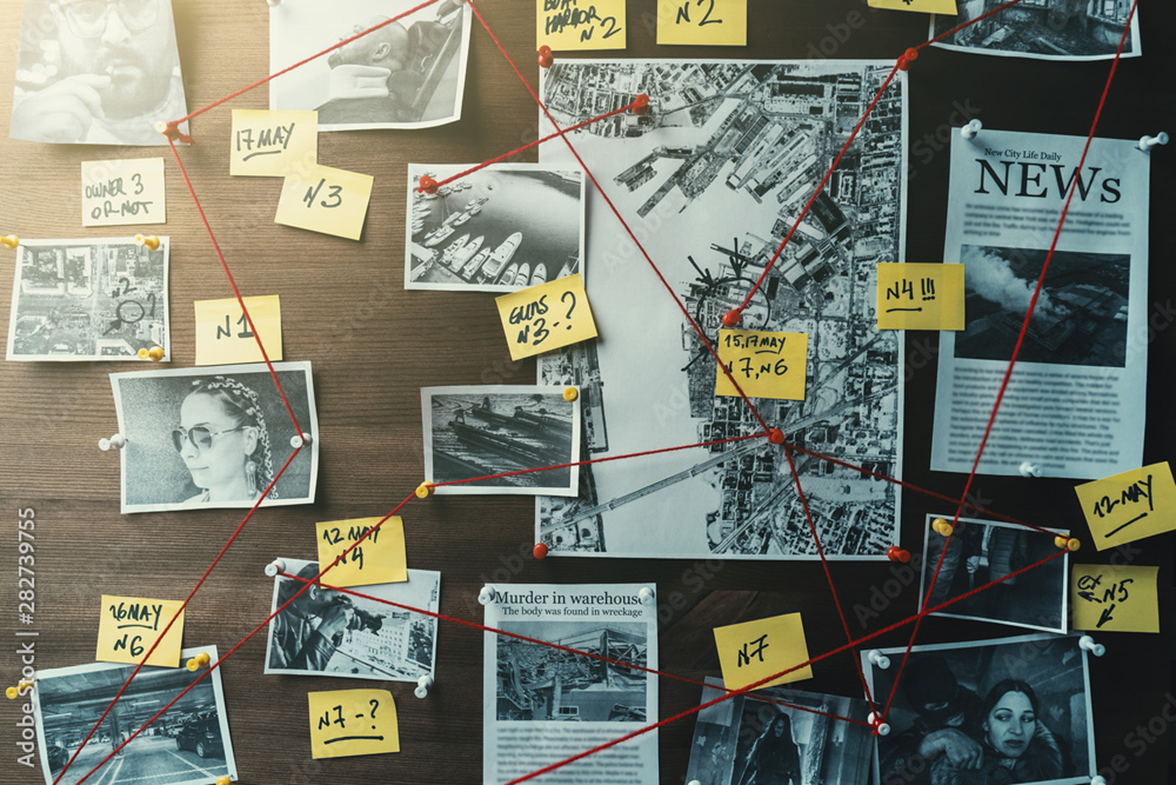
\includegraphics[width=1\textwidth]{images/crimediagramm.png}
    \caption{Crime diagram} \parencite{Neo4j:crimdiagram}
    \label{fig:crimeDiagram}
\end{figure}
\subsection{Nodes}
Nodes can be seen as the objects in a graph based database.
They can be tagged with labels (see section \ref{subsec:labels}) to describe their different roles and tasks in the graph model.
Nodes can also hold an arbitrary number of properties (see section \ref{subsec:properties}).
The following example shows two nodes with the label \("\)Person\("\), the properties \("\)name\("\), \("\)lastname\("\)
and \("\)email\("\) and their relationship to each other \parencite[compare P. 6f.]{PractivalNeo4j}.
\begin{figure}[!h]
    \centering
    \includegraphics[width=1 \linewidth]{images/node.png}
    \caption{Node sample} \label{img:cypher}
\end{figure}
\subsection{Relationships}\label{subsec:relationships}
Relationships provide connections between nodes.
They are named and can also have properties like nodes.
A single node can have multiple relationships to other nodes, these relationships can occur in any number or type without
sacrificing performance \parencite[compare]{neo4j:allgemeins}.

\subsection{Properties} \label{subsec:properties}
Properties are key-value pairs that can be attached to a node or a relationship.
Their purpose is to store metadata on them.
They can hold different types of data like strings, numbers, arrays, booleans, dates, times, points, and even other nodes and relationships \parencite[compare]{neo4j:Values} \parencite[compare]{neo4j:Graph}.

\subsection{Labels} \label{subsec:labels}
Labels can be seen as a way to group nodes.
Therefor a node with a specific label can provide additional values for each node.
For example, if you add a label called \("\)Student\("\) to a some nodes, they can have the same properties with different values.
A good example for this is the following graph model.
\begin{figure}[!h]
    \centering
    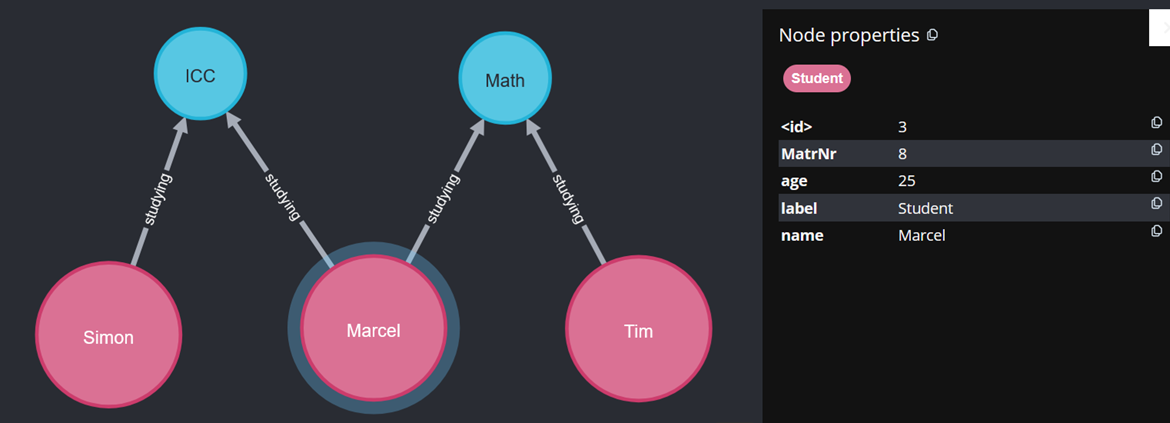
\includegraphics[width=1 \linewidth]{images/labels.png}
    \caption{Label sample} \label{img:labels}
\end{figure}
Labels are often used to show common subsets of essential node types.
Labels also offer a way to enforce modeling constraints when they are necessary, as well as increasing the speed at which data
can be accessed through improved indexing. \parencite[compare P. 6f.]{PractivalNeo4j}

\subsection{Traversal and indexing}\label{subsec:traversal-and-indexing}
Traversal is a common way of querying a graph in order to find a specific answer to a question or more precisely to find a
specific node or relationship.
The traversal is done by visiting nodes and following their relationships according to a set of specified rules \parencite[compare P.7]{PractivalNeo4j}.
This can be done in all sorts of algorithms, which can be roughly divided into two categories: breadth-first and depth-first.
The breadth-first  search begins with all neighboring nodes of the starting node and then continues with all neighbors of the neighboring nodes.
The depth-first search follows a path of the starting node until it reaches a dead end, then it backtracks and continues with the next path.
Explicit examples of traversal algorithms are the Hamiltonian path, the Eulerian path and the Dijkstra algorithm \parencite[compare]{juypiter:Graph}.
Indexing is also a way to find a specific node or relationship.
It is a way to speed up the search for a specific node or relationship by using specific indexes on a labeled node or relationship \parencite[compare P.7]{PractivalNeo4j}.